\documentclass[conference]{IEEEtran}
\IEEEoverridecommandlockouts
% The preceding line is only needed to identify funding in the first footnote. If that is unneeded, please comment it out.
\usepackage{cite}
\usepackage{amsmath,amssymb,amsfonts}
\usepackage{algorithmic}
\usepackage{graphicx}
\usepackage{textcomp}
\usepackage{xcolor}
\def\BibTeX{{\rm B\kern-.05em{\sc i\kern-.025em b}\kern-.08em
    T\kern-.1667em\lower.7ex\hbox{E}\kern-.125emX}}
\begin{document}

\title{Course Project of Numerical Analysis}

\author{\IEEEauthorblockN{Zhaohong Liu}
\IEEEauthorblockA{{ID: 122413910061} \\
}}

\maketitle



\section{Numerical Integration}

given that

$$
\int_0^R \rho v2 \pi r {\rm d}r
$$

with $\rho =1.2kg/m^3$

The first thing is to change unit from $m$ to $cm$ for $r$, 
then we use scatter to see the relation between $r$ and $v$.

\begin{figure}[htbp]
	\centerline{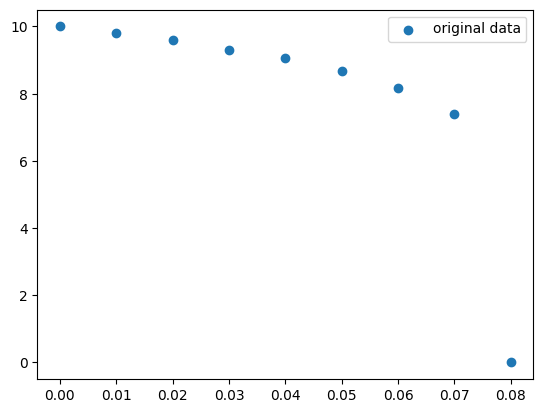
\includegraphics[width=0.85\columnwidth]{1-1.png}}
\end{figure}

It can be concluded that we can use interpolation methods to construct a polynomial,
which can be used in numerical integration.

So we use least square method to compose a fitting polynomial,

\begin{figure}[htbp]
	\centerline{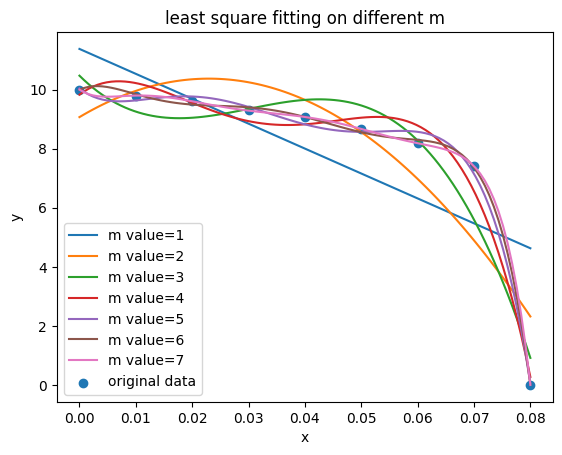
\includegraphics[width=0.9\columnwidth]{1-2.png}}
\end{figure}

The order can be as high as 7 if we wanted.
However, higher order doesn't equal to better efficiency, so order 5 is decided here.

Then we get the function, also the relation between $v$ and $r$.

$$
v(r) = 10 - 153r + 17677r^2 -70205r^3 + 13323135r^4 -80032051r^5 
$$

The next step is to compose $\rho v(r)2 \pi r$,
and coefficients for this function is:

[0.00000000e+00  7.57145786e+01 -1.15339684e+03  1.33281077e+05
-5.80721195e+06  1.00454071e+08 -6.03427440e+08]

Finally we use integration methods:
\begin{itemize}
	\item Composite trapezoidal rule: 0.1853
	\item Composite Simpson's rule: 0.1855
	\item Romberg's method(order 10): 0.1855 
\end{itemize}

\section{ODE Initial Value Problem}

given that

$$
\frac{\partial k}{\partial t} = -\epsilon
$$

and

$$
\frac{\partial \epsilon}{\partial t} = -C \frac{\epsilon^2}{k}
$$

where $C=1.83$. At $t_0=1,\quad k=1,\quad \epsilon=0.2176$

predict $k$ at $t=5$

For each step, firstly we use ${\partial \epsilon}/{\partial t}$ to get $\epsilon(t)$;
secondly send this $\epsilon(t)$ into ${\partial k}/{\partial t}$ to acquire the $k$.

The final is:
\begin{itemize}
	\item Euler's method: 0.490872
	\item Modified Euler's method: 0.472633
	\item Runge-Kutta 4: 0.473380
\end{itemize}

Considering both convergence and accuracy, euler's method should be the last one of the three methods,
while modified euler method works better than euler's method;

The most fast-converge and accurate method of the three should be 4-th runge kutta method.

\section{Non Linear Equations}
given that
$$
y_+ = U_+ + e^{-kB} [e^{kU_+} - 1 - kU_+ - \frac12(kU_+)^2 - \frac16(kU_+)^3 - \frac{1}{24}(kU_+)^4]
$$

where

$$
y_+ = \frac{u_ry}{v}, \quad U_+=\frac{U}{u_r}
$$

$$
k=0.41, \quad B=5.1, \quad v=1.5\times 10^{-5}, \quad \rho=1.25 kg/m^3
$$

$y=0.01m$, the velocity is $21m/s$

$$
u_{\tau} = \sqrt{\frac{\tau_{wall}}{\rho}}
$$

The first step is to use matplotlib.pyplot to find box of root.

\begin{figure}[htbp]
	\centerline{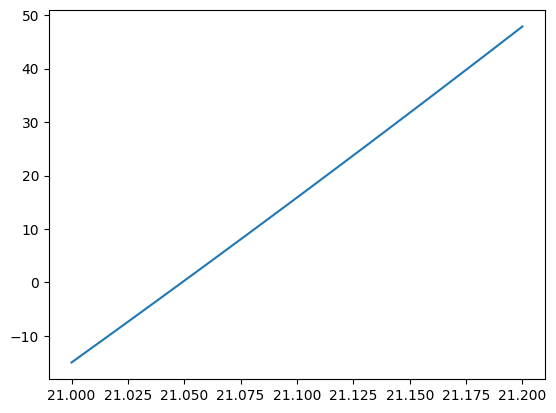
\includegraphics[width=0.9\columnwidth]{3-1.png}}
\end{figure}

so the initial guess value can be set as 21.

Then applying three methods to get $U_+$:

\begin{itemize}
	\item Bisection method: 21.0498
	\item Newton method: 21.0494
	\item Fix point method: 21.0498
\end{itemize}

we can then conclude that $\tau_{wall} = 1.2441$

and the formula for Fix point method is:

$$
U_+ = g(U_+) = ln((y_+ + U_+)e^{kB} + 1 + kU_+ + \frac12(kU_+)^2
$$

$$
 + \frac16(kU_+)^3 + \frac{1}{24}(kU_+)^4) / k
$$

\section{Interpolation}

\begin{figure}[htbp]
	\centerline{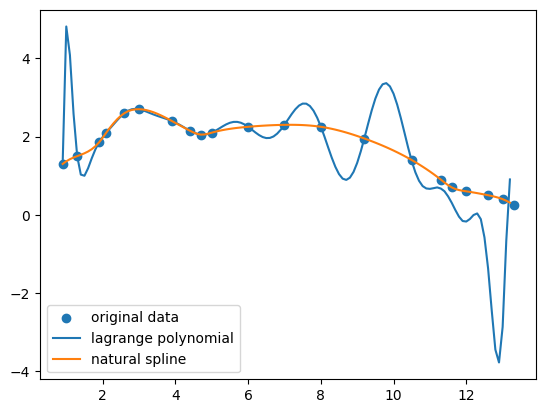
\includegraphics[width=0.9\columnwidth]{4-1.png}}
\end{figure}

With many as 21 points, the lagrange method could not follow the trend of original data points.

However, the natural spline function basically keeps the same changing pattern as original data points go.

\section{Linear Equations}

gaussian elimination:  [-9.62900109e+03  5.23308734e+04 -1.28353328e+05  1.89495703e+05
-1.89338391e+05  1.36397396e+05 -7.36542206e+04  3.05862459e+04
-9.93812152e+03  2.55593429e+03 -5.24043290e+02  8.59478924e+01
-1.12743546e+01  1.17827153e+00 -9.72945654e-02  6.25917429e-03
-3.06784319e-04  1.10555985e-05 -2.75922145e-07  4.25747987e-09
-3.05797637e-11]


LU decomposition:  [-9.60454784e+03  5.21953487e+04 -1.28013353e+05  1.88980865e+05
-1.88809167e+05  1.36003965e+05 -7.34343002e+04  3.04914228e+04
-9.90603943e+03  2.54731981e+03 -5.22194910e+02  8.56299984e+01
-1.12305538e+01  1.17345714e+00 -9.68760682e-02  6.23081593e-03
-3.05319883e-04  1.09999978e-05 -2.74460563e-07  4.23373827e-09
-3.04003669e-11]


gauss-seidel:  [[-5.34167848e+04]
[ 1.51689637e+05]
[-1.81222598e+05]
[ 1.81139810e+05]
[-1.86383242e+05]
[ 1.42524271e+05]
[-7.54223407e+04]
[ 3.04691827e+04]
[-9.96721192e+03]
[ 2.58850592e+03]
[-5.25063148e+02]
[ 8.49677686e+01]
[-1.11779782e+01]
[ 1.18017590e+00]
[-9.78315352e-02]
[ 6.30218484e-03]
[-3.09533404e-04]
[ 1.10590396e-05]
[-2.74274036e-07]
[ 4.44400390e-09]
[-2.96942589e-11]]


SOR:  [[-5.34167848e+04]
[ 1.51689637e+05]
[-1.81222598e+05]
[ 1.81139810e+05]
[-1.86383242e+05]
[ 1.42524271e+05]
[-7.54223407e+04]
[ 3.04691827e+04]
[-9.96721192e+03]
[ 2.58850592e+03]
[-5.25063148e+02]
[ 8.49677686e+01]
[-1.11779782e+01]
[ 1.18017590e+00]
[-9.78315352e-02]
[ 6.30218484e-03]
[-3.09533404e-04]
[ 1.10590396e-05]
[-2.74274036e-07]
[ 4.44400390e-09]
[-2.96942589e-11]]

\section{Eigen Value}

$$
A = \begin{bmatrix}
52 & 30 & 49 & 28\\
30 & 50 & 8 & 44\\
49 & 8 & 46 & 16\\
28 & 44 & 16 & 22
\end{bmatrix}
$$

Power iteration: Max eigen value =  [132.94900421]

Rayleigh quotient: Max eigen value =  [[132.62787533]]

QR decomposition, eigen values =  [132.62759169  52.4425832  -11.54109674  -3.52907815]


\end{document}
